\documentclass[tikz,border=8pt]{standalone}
\usetikzlibrary{arrows.meta,positioning}
\begin{document}
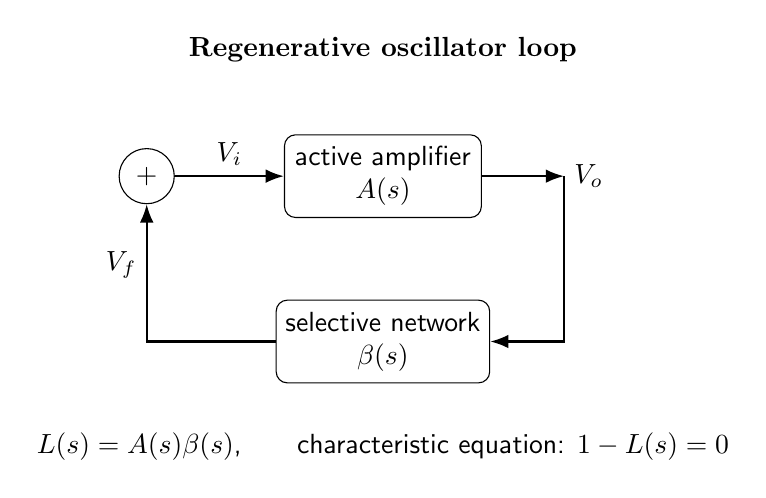
\begin{tikzpicture}[>=Latex,font=\sffamily,block/.style={draw,rounded corners,minimum width=2.5cm,minimum height=1.05cm,align=center},line/.style={->,thick}]
\node[circle,draw,minimum size=7mm] (sum) at (0,0) {$+$};
\node[block] (amp) at (3,0) {active amplifier\\$A(s)$};
\node[block] (net) at (3,-2.1) {selective network\\$\beta(s)$};
\draw[line] (sum) -- node[above]{$V_i$} (amp);
\draw[line] (amp) -- ++(2.3,0) coordinate(out) node[right]{$V_o$};
\draw[line] (out) |- (net.east);
\draw[line] (net.west) -| node[pos=.78,left]{$V_f$} (sum.south);
\node[above=8mm of amp,font=\bfseries] {Regenerative oscillator loop};
\node[below=5mm of net,align=center] {$L(s)=A(s)\beta(s)$,\qquad characteristic equation: $1-L(s)=0$};
\end{tikzpicture}
\end{document}
